\section{Empirical study}
This section will be dedicated to the results of the first research question: \textit{What is the current state of the art and what is the performance
of these tools?}. The tools that have been selected to represent the state of the art have been discussed in both chapter \ref{chap:background} and \ref{chap:methodology}. The results will now dive into the second part of the research question, as the performance results from the empirical study executed will be presented below. 

\paragraph{Specs}
All the experiments were run on 
Experiments were run on a computer with an Intel Core i7 8750H processor using 16 GB of RAM, running Ubuntu 18.04 as Windows Subsystem for Linux 2. % running at 2.20 GHz base, 4.1 GHz max 
The max runtime for a single experiment was limited at 1800 seconds (half hour). A timeout error would occur after that and the experiment would be canceled. 

\subsection{Error detection tool configurations}
After generating configurations with the settings shown in \ref{sec:empiricalstudy}, the number of strategies per tool are shown in table \ref{tab:number_configs_tool}. 

\begin{table}[H]
\centering
\begin{tabular}{lr}
\toprule
Tool &  Number of strategies \\
\midrule
dBoost            &                  72 \\
Raha              &                  37 \\
ForbiddenItemSets &                   7 \\
ActiveClean       &                   7 \\
KATARA            &                   4 \\
FAHES             &                   4 \\
\bottomrule
\end{tabular}
\caption{Number of configurations per tool}
\label{tab:number_configs_tool}
\end{table}

With the set timeout and input parameters, not all strategies are able to generate a correct output. In table \ref{tab:number_configs_tool}, the number of strategies and the number of correct results they produced are shown. On the left, the amount of correct results the strategy returned and on the right, the number of strategies that have returned that number of results. Meaning that 103 strategies were able to provide output for all the datasets. There were 2 and 1 strategies able to return results for 13 and 12 datasets respectively. Then, there was a gap, mainly caused by strategies that had multiple timeouts or other errors for example caused by memory limits.

\begin{figure}
    \centering
    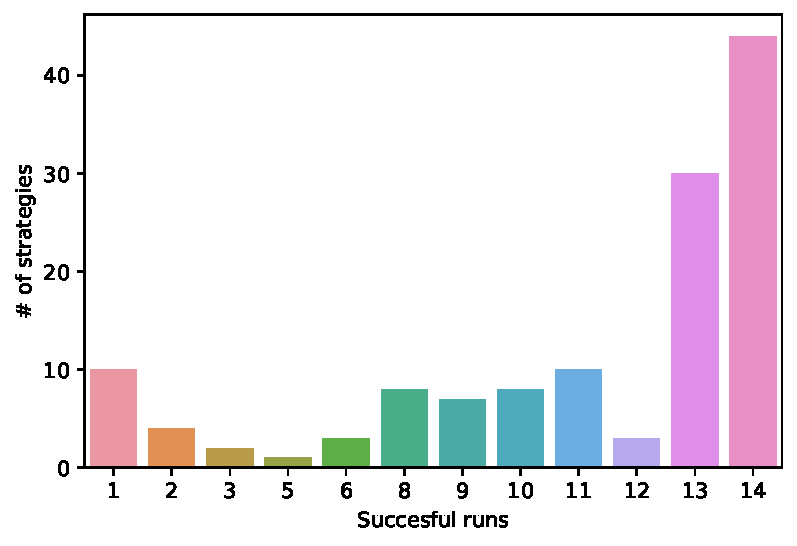
\includegraphics[width=0.8\linewidth]{thesis/Figures/RQ2/SuccesfulRuns.pdf}
    \caption{Number of strategies per total completed runs}
    \label{fig:number_configs_runs}
\end{figure}

\subsection{Results}
An aggregate of all the performance scores is shown in table \ref{tab:empirical_results}. All human-aided tools with a maximum of 20 (perfectly accurate) human interactions and all the other non-human interactive tools are used in this aggregate. Then, the performance scores with the highest F1-score for all configurations of a tool is kept per dataset. Precision, recall and the F1-score are shown from left to right per column. The best score for each dataset is marked bold.

\begin{table}[H]
\centering
\caption{|Precision Recall F1-score| for tool as column \& dataset as row}
\label{tab:empirical_results}
\begin{adjustbox}{center}
\begin{tabular}{lllllll}
\toprule
{} & ActiveClean & FAHES & ForbiddenItemSets & KATARA & Raha & dBoost \\
\midrule
 & \textbf{\space\space\space P \space\space\space\space R \space\space\space F1} & \textbf{\space\space\space P \space\space\space\space R \space\space\space F1} & \textbf{\space\space\space P \space\space\space\space R \space\space\space F1} & \textbf{\space\space\space P \space\space\space\space R \space\space\space F1} & \textbf{\space\space\space P \space\space\space\space R \space\space\space F1} & \textbf{\space\space\space P \space\space\space\space R \space\space\space F1} \\
airbnb & 0.15 \textbf{1.00} 0.26 & \textbf{0.54} 0.01 0.02 & 0.13 0.29 0.18 & Other error & 0.42 0.13 0.20 & 0.23 0.38 \textbf{0.28} \\
beers & 0.16 \textbf{1.00} 0.28 & 0.83 0.02 0.04 & 0.34 0.30 0.32 & 0.14 0.26 0.18 & \textbf{0.97} 0.69 \textbf{0.80} & 0.68 0.55 0.61 \\
eeg & 0.04 0.03 0.03 & 0.00 0.00 0.00 & 0.02 0.26 0.04 & 0.00 0.00 0.00 & \textbf{0.56} 0.71 \textbf{0.63} & 0.13 \textbf{1.00} 0.23 \\
flights & 0.30 \textbf{0.98} 0.46 & 0.23 0.01 0.02 & 0.56 0.16 0.24 & 0.09 0.09 0.09 & 0.90 0.83 \textbf{0.86} & \textbf{0.94} 0.59 0.72 \\
hospital & 0.03 0.47 0.05 & 0.02 0.09 0.04 & 0.01 0.06 0.02 & 0.08 0.37 0.13 & \textbf{0.98} \textbf{0.57} \textbf{0.72} & 0.03 0.43 0.06 \\
marketing & 0.25 0.36 0.30 & 0.24 0.01 0.01 & 0.25 0.46 0.33 & 0.21 0.32 0.25 & \textbf{0.50} 0.32 0.39 & 0.34 \textbf{0.67} \textbf{0.45} \\
movie & 0.37 \textbf{1.00} 0.54 & 0.00 0.00 0.00 & 0.31 0.08 0.13 & 0.43 0.43 0.43 & \textbf{0.47} 0.64 \textbf{0.54} & 0.37 \textbf{1.00} 0.54 \\
movies & 0.02 0.00 0.01 & 0.01 0.10 0.02 & 0.01 0.06 0.01 & 0.02 0.16 0.03 & \textbf{0.72} \textbf{0.76} \textbf{0.74} & 0.01 0.09 0.03 \\
rayyan & 0.09 \textbf{1.00} 0.16 & 0.07 0.04 0.05 & Other error & 0.01 0.02 0.01 & \textbf{0.86} 0.84 \textbf{0.85} & 0.22 0.77 0.34 \\
restaurant & 0.01 \textbf{0.83} 0.02 & 0.00 0.00 0.00 & 0.01 0.07 0.01 & 0.00 0.13 0.01 & \textbf{0.14} 0.11 \textbf{0.12} & 0.03 0.03 0.03 \\
restaurants & 0.00 0.00 0.00 & \textbf{0.00} 0.07 \textbf{0.01} & Other error & 0.00 0.22 0.00 & 0.00 \textbf{1.00} 0.00 & 0.00 0.08 0.00 \\
toy & Other error & 0.00 0.00 0.00 & 0.00 0.00 0.00 & 0.21 0.75 0.33 & 0.22 \textbf{1.00} 0.36 & \textbf{0.33} 0.75 \textbf{0.50} \\
university & 0.03 0.09 0.04 & 0.00 0.00 0.00 & Other error & 0.06 0.29 0.10 & \textbf{0.99} 0.91 \textbf{0.95} & 0.32 \textbf{1.00} 0.49 \\
uscensus & 0.02 0.00 0.00 & 0.01 0.18 0.02 & 0.02 0.26 0.04 & 0.00 0.00 0.00 & \textbf{1.00} \textbf{1.00} \textbf{1.00} & 0.41 \textbf{1.00} 0.58 \\
\bottomrule
\end{tabular}
\end{adjustbox}
\end{table}

The results above are also shown as boxplots in figure \ref{fig:f1_boxplot} to show a direct overview of the best performing configurations per tool, measured by the F1 score. From the table and figures shown, the conclusion can be drawn that Raha performs best overall for all the tools. Because Raha makes use of different underlying error detection techniques, it is capable of detecting a wide range of errors. In this setup were the error detection task was to detect not only specific errors, but all sorts, the more general methods perform better.
% Non human expert
\\From the non-interactive tools, dBoost performs the best. Without being able to find rule violations, the tool still manages to perform well overall. This might mean that in the datasets used, more errors were detectable using pattern violations or outliers. 
Besides Raha, the other human interactive tool ActiveClean is the next best tool on average. However, this tool mostly scores best when marking all the values as errors, when the datasets have relatively more errors, like dataset movie or flights (see statistics in table \ref{tab:dataset_statistics}). The last tools, FAHES, ForbiddenItemSets and KATARA perform worst overall. FAHES is a relatively specific tool, as it mainly tries to find disguised missing values. It could maybe fit in the data cleaning pipeline somewhere where only the missing values need to be detected. ForbiddenItemSets scores a decent average F1-score, as shown in figure \ref{fig:f1_boxplot}, but does not cut it against the top 3. It does have higher precision than FAHES and KATARA overall, making it maybe possible to use in automated fashion, or as submodule in a composite method like Raha. Lastly, KATARA also performs below average. This is due to the fact that KATARA is highly dependent on the domain the dataset has and the domain given to KATARA as knowledge base. Apparently, the combination of knowledge base parts was not suited well enough for the test datasets.

\begin{figure}
\centering
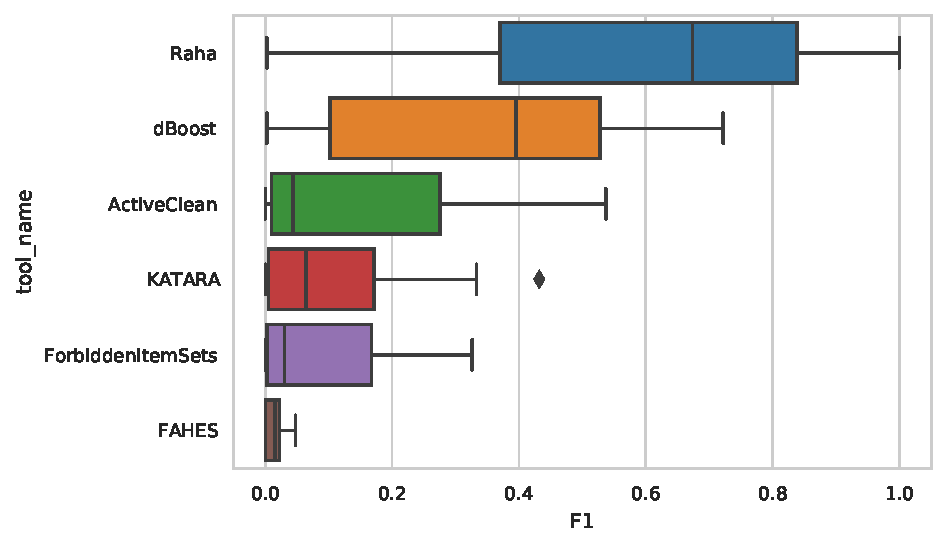
\includegraphics[width=0.9\textwidth]{Figures/RQ1/F1Boxplot.pdf}
\caption{F1 boxplots for the best tool results}
\label{fig:f1_boxplot}
\end{figure}

\paragraph{Execution times} 
Beside the performance scores in figure \ref{fig:f1_boxplot} and table \ref{tab:empirical_results}, the execution times in seconds of the best configuration are visualized in figure \ref{fig:runtime_boxplot}. Raha does have the best performance scores overall, but also takes the most time to execute. Raha is a composite method and uses the result of multiple simpler error detection methods. Consequently, the runtime also depends greatly on the underlying methods. So the sum of all the underlying error detection strategies make it so that it is also the most time consuming tool. The second best tool, dBoost, has a lesser median runtime than most tools, but has some outliers for larger datasets. In general, the case is that these error detection tools are worse than linearly correlated to the input size with respect to runtime. 

\begin{figure}
    \centering
    \begin{adjustbox}{center}
    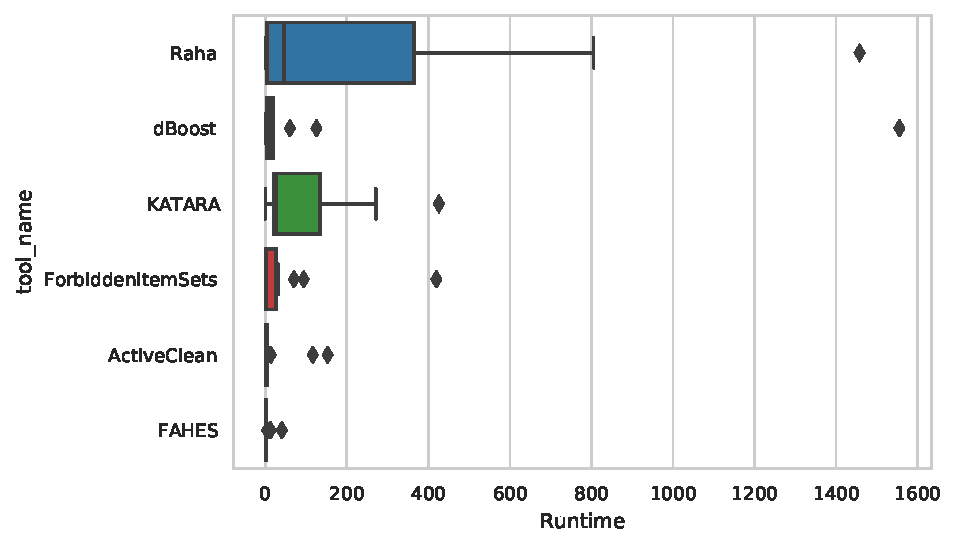
\includegraphics[width=\linewidth]{thesis/Figures/RQ1/RuntimeBoxplot.pdf}
    \end{adjustbox}
    \caption{Boxplot of the runtime in seconds for the best tool results}
    \label{fig:runtime_boxplot}
\end{figure}


\paragraph{No human interaction} In the previous section, it has been shown that Raha performs best out of the 6 implemented tools. But, Raha is depending on user labeling. This means that the end-user of this error detection tool should be able to differentiate errors from the ground truth. If such a domain expert is not available, strategies without human interaction could be of interest. In table \ref{tab:empirical_results_no_human}, the same aggregated best (highest F1-score) performance scores for each tool per dataset are shown. The ActiveClean implementation does not have a configuration without human interaction. Raha does, but the best performing strategies were the ones that simply marked all cells as errors. Concluding from this table, it can be said that if there is not a user who can do the labeling for the domain of that dataset, dBoost will be the best solution to use.

\begin{table}
\centering
\caption{|Precision Recall F1-score| for tool as column \& dataset as row \textbf{without human interaction}}
\label{tab:empirical_results_no_human}
\begin{adjustbox}{center}
\begin{tabular}{llllll}
\toprule
{} & FAHES & ForbiddenItemSets & KATARA & Raha & dBoost \\
\midrule
 & \textbf{\space\space\space P \space\space\space\space R \space\space\space F1} & \textbf{\space\space\space P \space\space\space\space R \space\space\space F1} & \textbf{\space\space\space P \space\space\space\space R \space\space\space F1} & \textbf{\space\space\space P \space\space\space\space R \space\space\space F1} & \textbf{\space\space\space P \space\space\space\space R \space\space\space F1} \\
airbnb & \textbf{0.54} 0.01 0.02 & 0.13 0.29 0.18 & Other error & Other error & 0.23 \textbf{0.38} \textbf{0.28} \\
beers & \textbf{0.83} 0.02 0.04 & 0.34 0.30 0.32 & 0.14 0.26 0.18 & 0.16 \textbf{1.00} 0.28 & 0.68 0.55 \textbf{0.61} \\
eeg & 0.00 0.00 0.00 & 0.02 0.26 0.04 & 0.00 0.00 0.00 & Other error & \textbf{0.13} \textbf{1.00} \textbf{0.23} \\
flights & 0.23 0.01 0.02 & 0.56 0.16 0.24 & 0.09 0.09 0.09 & 0.30 \textbf{1.00} 0.46 & \textbf{0.94} 0.59 \textbf{0.72} \\
hospital & 0.02 0.09 0.04 & 0.01 0.06 0.02 & \textbf{0.08} 0.37 \textbf{0.13} & 0.03 \textbf{1.00} 0.05 & 0.03 0.43 0.06 \\
marketing & 0.24 0.01 0.01 & 0.25 0.46 0.33 & 0.21 0.32 0.25 & Other error & \textbf{0.34} \textbf{0.67} \textbf{0.45} \\
movie & 0.00 0.00 0.00 & 0.31 0.08 0.13 & \textbf{0.43} 0.43 0.43 & Other error & 0.37 \textbf{1.00} \textbf{0.54} \\
movies & 0.01 0.10 0.02 & 0.01 0.06 0.01 & \textbf{0.02} 0.16 \textbf{0.03} & 0.01 \textbf{1.00} 0.02 & 0.01 0.09 0.03 \\
rayyan & 0.07 0.04 0.05 & Other error & 0.01 0.02 0.01 & 0.09 \textbf{1.00} 0.16 & \textbf{0.22} 0.77 \textbf{0.34} \\
restaurant & 0.00 0.00 0.00 & 0.01 0.07 0.01 & 0.00 0.13 0.01 & 0.00 \textbf{1.00} 0.01 & \textbf{0.03} 0.03 \textbf{0.03} \\
restaurants & \textbf{0.00} 0.07 \textbf{0.01} & Other error & 0.00 0.22 0.00 & 0.00 \textbf{1.00} 0.00 & 0.00 0.08 0.00 \\
toy & 0.00 0.00 0.00 & 0.00 0.00 0.00 & 0.21 0.75 0.33 & 0.22 \textbf{1.00} 0.36 & \textbf{0.33} 0.75 \textbf{0.50} \\
university & 0.00 0.00 0.00 & Other error & 0.06 0.29 0.10 & 0.03 \textbf{1.00} 0.05 & \textbf{0.32} \textbf{1.00} \textbf{0.49} \\
uscensus & 0.01 0.18 0.02 & 0.02 0.26 0.04 & 0.00 0.00 0.00 & Other error & \textbf{0.41} \textbf{1.00} \textbf{0.58} \\
\bottomrule
\end{tabular}
\end{adjustbox}
\end{table}

% What if the best tool has 0.75 human expertise?
\paragraph{Inaccurate human labeling} If there is a user willing and able to actively label cells during error detection, there still remains the question of how accurate those labels are. To show the implications of lesser accurate labeling, all the configuration of Raha were executed again, but the human interactions were simulated to be only 75\% accurate, in stead of 100\%. The results are shown in table \ref{tab:raha_empirical}, with the fully accurate labeling on the left side, and the 75\% accuracy on the rights side. Immediately can be seen that tool is highly dependent on human accuracy. Only for 1 out of the 14 datasets, the tool randomly performed better with lower labeling accuracy according to the F1-score, then it did with full accuracy, due to the randomness in Raha. But precision-wise, for none of the datasets, the less accurate experiments produced better results than the fully accurate strategies. A user of interactive error detection tools should take this into account when deciding for an error detection tool. Solutions like repeated labeling by users could maybe mitigate the risk (as examples have shown by \cite{Sheng2008-gk}).

\begin{table}
\centering
\caption{|Precision Recall F1-score| for Raha with different human labeling accuracy}
\label{tab:raha_empirical}
\begin{tabular}{lll}
\toprule
{} & Raha 100\% & Raha 75\% \\
\midrule
 & \textbf{\space\space\space P \space\space\space\space R \space\space\space F1} & \textbf{\space\space\space P \space\space\space\space R \space\space\space F1} \\
airbnb & \textbf{0.42} 0.13 0.20 & 0.19 \textbf{0.36} \textbf{0.25} \\
beers & \textbf{0.97} 0.69 \textbf{0.80} & 0.70 \textbf{0.81} 0.75 \\
eeg & \textbf{0.56} \textbf{0.71} \textbf{0.63} & 0.10 0.44 0.16 \\
flights & \textbf{0.90} \textbf{0.83} \textbf{0.86} & 0.60 0.73 0.66 \\
hospital & \textbf{0.98} \textbf{0.57} \textbf{0.72} & 0.09 0.54 0.15 \\
marketing & \textbf{0.50} 0.32 \textbf{0.39} & 0.30 \textbf{0.47} 0.37 \\
movie & \textbf{0.47} 0.64 \textbf{0.54} & 0.41 \textbf{0.71} 0.52 \\
movies & \textbf{0.72} \textbf{0.76} \textbf{0.74} & 0.11 0.35 0.17 \\
rayyan & \textbf{0.86} 0.84 \textbf{0.85} & 0.71 \textbf{0.84} 0.77 \\
restaurant & \textbf{0.14} 0.11 \textbf{0.12} & 0.01 \textbf{0.58} 0.03 \\
restaurants & \textbf{0.00} \textbf{1.00} \textbf{0.00} & 0.00 0.00 0.00 \\
toy & \textbf{0.22} \textbf{1.00} \textbf{0.36} & Other error \\
university & \textbf{0.99} \textbf{0.91} \textbf{0.95} & 0.25 0.78 0.38 \\
uscensus & \textbf{1.00} \textbf{1.00} \textbf{1.00} & 0.05 0.64 0.09 \\
\bottomrule
\end{tabular}
\end{table}